\documentclass[12pt]{article}

\addtolength{\textwidth}{1.3in}
\addtolength{\oddsidemargin}{-.65in} %left margin
\addtolength{\evensidemargin}{-.65in}
\setlength{\textheight}{9in}
\setlength{\topmargin}{-.5in}
\setlength{\headheight}{0.0in}
\setlength{\footskip}{.375in}
\renewcommand{\baselinestretch}{1.0}
\linespread{1.5}

\usepackage[backend=biber,block=space,style=authoryear-comp]{biblatex}

%campus computer
%\usepackage[backend=bibtex,block=space,style=authoryear]{biblatex}

%dell laptop
\addbibresource{C:/Users/Kristy/Dropbox/Research/xBibs/tradeagreements.bib}

%campus computer
\addbibresource{C:/Apps-SU/Dropbox/Research/xBibs/tradeagreements.bib}
\renewcommand{\newunitpunct}{,}
\renewbibmacro{in:}{}

\usepackage{csquotes}
\setlength{\bibitemsep}{\baselineskip}
\usepackage[american]{babel}
\usepackage[usenames,dvipsnames]{color}
\usepackage{tikz}
\tikzset{
% Two node styles for game trees: solid and hollow
solid node/.style={circle,draw,inner sep=1.5,fill=black},
hollow node/.style={circle,draw,inner sep=1.5,fill=white}
%non node/.style={circle,draw,inner sep=.1,fill=black}
}

\usepackage[pdftex,
bookmarks=true,
bookmarksnumbered=false,
pdfview=fitH,
bookmarksopen=true,hyperfootnotes=false]{hyperref}
\usepackage{graphicx}

\usepackage{amsbsy,amssymb, amsmath, amsthm, MnSymbol,bbding}
\usepackage[hang,flushmargin]{footmisc} 

%\usepackage{cite}
\usepackage{times, verbatim,bm,pifont,pdfsync}
%\usepackage[hang,flushmargin]{footmisc}%unindents footnotes

% disables chapter, section and subsection numbering
%\setcounter{secnumdepth}{-1} 

\newtheorem{definition}{Definition}
\newtheorem{theorem}{Theorem}
\newtheorem{lemma}{Lemma}
\newtheorem{corollary}{Corollary}
\newtheorem{assumption}{Assumption}
\newtheorem{fact}{Fact}
\newtheorem{result}{Result}
\newtheorem{proposition}{Proposition}

\newcommand{\ve}{\theta}
\newcommand{\ta}{\theta}
\newcommand{\ov}{\overline}
\newcommand{\un}{\underline}
\newcommand{\al}{\alpha}
\newcommand{\Ta}{\Theta}
\newcommand{\expect}{\mathbb{E}}
\newcommand{\Bt}{B(\bm{\tau^a})}
\newcommand{\bta}{\bm{\tau^a}}
\newcommand{\bte}{\bm{\tau^E}}
\newcommand{\btn}{\bm{\tau^n}}
\newcommand{\ga}{\gamma}
\newcommand{\btw}{\bm{\tau^{tw}}}
\newcommand{\de}{\delta}

%This version was begun on May 10, 2014 for first public release (to ISNIE posting and first posting to my website); I anticipate those main changes will be some significant editing since first draft for Midwest was hurried, plus some expansion to escape clause section.

\begin{document}
\title{Endogenous Politics and the Design of Trade Institutions\thanks{I thank Kyle Bagwell, Mostafa Beshkar, Rick Bond, Renee Bowen, Chad Bown, Paola Conconi, David DeRemer, James Lake, Nuno Limao, Giovanni Maggi, Devashish Mitra, Peter Rosendorff, Bob Staiger, Maurizio Zanardi, Ben Zissimos and participants in seminars at McGill, Rochester, Ryerson, Wesleyan, ETSG, InsTED, the Midwest International Trade Meetings, PEIO and SITE for very helpful comments and discussions.}}
\author{Kristy Buzard\thanks{Syracuse University, Economics Department. Email: kbuzard@syr.edu. http://faculty.maxwell.syr.edu/kbuzard.}}
\date{\vskip-.1in \today}
\maketitle

\vskip.3in
\begin{center} {\bf Abstract} \end{center}

\begin{quote}
{\small Political pressure is undoubtedly an important influence in the formulation of trade agreements and the institutions that govern them. Much of the literature that speaks to the design of trade policy institutions takes the political pressure that governments face as resulting from an exogenous, stochastic process. This paper shows that when political pressure arises endogenously, important results may be overturned and new insights into the motivation for features of the trade agreements we observe and rules of organizations such as the WTO come to light. Developing a model that integrates both exogenous and endogenous political pressure and taking a general approach to the government objective function, I show that governments may want to use tariff caps both to force special interest groups to continue lobbying after a trade agreement is signed and to reduce the magnitude of that lobbying effort. The presence of endogenous politics can also destroy the ability of an escape clause as traditionally defined in the literature to provide flexibility in times of large negative political shocks when lobbies use the flexibility to seek rents. This can explain why the use of WTO Safeguards are conditioned on measurable economic indicators.}
\end{quote}

%JEL Codes: F13,F53,C73,D72

\bigskip
\section{Introduction}
Much of the work on the political economy of trade agreements focuses on questions regarding the optimal design of trade agreements, trade agreement negotiations, and trade dispute settlement that arise in the presence of asymmetric information about shocks to an exogenous political economy parameter. That political economy forces are entirely driven by exogenous forces is a rather drastic simplifying assumption. Do the predictions of our models hold up if this simplifying assumption is relaxed?

One of the basic ideas that emerges from this literature is that in the presence of asymmetric information about the strength of the ex-post political economy shocks, it is often advantageous to grant governments a period of relief from trade commitments. That is, one would rather allow a short period of ``escape'' from the agreement rather than have the agreement violated because domestic political opposition is temporarily too strong to be resisted.

This is an intuitively appealing story, but the logic can break down in the presence of endogenous political pressure. An escape clause allows a government to apply a higher tariff barrier when it experiences intense political pressure. But if a government gets a free pass at the WTO whenever it feels sufficient political pressure from domestic interest groups, those interest groups have a strong incentive to exert the required level of pressure regardless of the underlying state of the world, eviscerating the escape clause.

This is one example of a design question whose answers are sensitive to assumptions about the endogeneity of political pressure. In order to examine this question and others, I use a simple model that is standard in the literature (e.g. \Textcite{bs2001}, \Textcite{bown2002}, \Textcite{bown2004}, \Textcite{bs2005}, \Textcite{martinvergote}, \Textcite{bagwell2009}, \Textcite{beshkar2010a}, \Textcite{ms2012a}, and \Textcite{ms2013}) and add an endogenously-determined element to the usual exogenously-determined political economy weights. Because of its tractability, this model can address a wide range of institutional design questions while also allowing endogenous politics to be taken into account in a repeated-game setting.\footnote{Repeated non-cooperative-game models of trade agreements have been considered by \Textcite{mcm86,mcm89}, \Textcite{dixit1987}, \Textcite{bs1990, bs1997a, bs1997b, bs2002}, \Textcite{kovthurs}, \Textcite{maggi99}, \Textcite{coatesludema}, \Textcite{ederington}, \Textcite{rosendorff}, \Textcite{bagwell2009}, and \Textcite{park}. \Textcite{buzard2013a} features a repeated-game model similar in spirit to the model under consideration here but focusing on questions of optimal punishments when the government is non-unitary.}

I first establish the baseline case with tariff caps and no escape clause. Here, I find that the presence of endogenous political pressure changes the optimal choice of tariff bindings within a trade agreement in quite significant ways compared with the case where political pressure is assumed to be exogenous, and that endogenous political pressure makes it harder to incentivize cooperation through repeated game incentives. As in \Textcite{mrc2007}, I show in this simpler framework that allows for easy comparison to the exogenous shocks case that one of the uses of tariff caps is to incentivize the lobby to engage in the political process after the trade agreement is in place. Combined with the idea that governments can use tariff caps to restrain endogenous political pressure, a story emerges in which governments employ trade agreements to carefully manipulate lobbying incentives in order to maximize their political objectives.

In order to make this point clear, I compare political welfare under the standard \Textcite{baldwin}-style government objective function to political welfare under the government objective function I introduce that takes account of endogenous politics. In my formulation, the government is not necessarily always better off as political pressure climbs higher and higher, while the \Textcite{baldwin}-style  government objective function is everywhere increasing in political pressure. \Textcite{gh94} and its extension to trade agreements in \Textcite{gh95} provide microfoundations for this \Textcite{baldwin}-style government objective function, where a fixed weight of $1+a$ is attached to the surplus of groups who lobby, and $a$ to the surplus of those who don't lobby.\footnote{Note that $a$ is the weight the government places on social welfare.} This cannot microfound a flexible model as in \Textcite{longvousden} or in which shocks to the political-economy weights come from shocks to any parameter other than the weight the government places on social welfare.

More importantly, this standard functional form leads inexorably to the conclusion that governments do not want to discourage political pressure except in the presence of long-run inefficiencies such as in \Textcite{mitra} and \Textcite{mrc2007}. The modification to the government objective function I propose leads to the result that governments may indeed want to use trade agreements to reduce lobbying in many environments.\footnote{With only one lobby in each country, the governments will be unable to encourage lobbying in excess of that which is optimal from the lobby's point of view.} Examining this alternative welfare function in combination with endogenous lobbying can provide a bridge between the theoretical literature and the claims of trade policy practitioners that an important role of trade agreements is to rein in protectionist pressure.

In the main example of this paper, I show that the same combination---endogenously-determined political pressure and a general approach to the government's objective function---can explain why the conditions for invoking the WTO Safeguards measure rely on purely observable economic variables, and why the level of protection governments can choose when invoking a Safeguard is related to the injury imposed by the shock and not its political impact. The model formalizes the intuition that if the WTO's Dispute Settlement Body actually followed the procedures suggested by the literature---that is, it enforced commitments based on signals of the political pressure experienced by governments---pressure groups would simply exert more pressure and the Safeguard clause could not play the escape-providing role for which it was intended. On the other hand, if the purpose of contingent protection measures is actually to provide a political safety valve, this analysis could help explain the infrequency with which safeguards are invoked under the WTO, as I argue that the WTO's escape clause has been designed to provide relief only from economic shocks.

We miss important dynamics like this one when we assume political pressure is exogenous as is done for tractability in almost all the literature that studies trading rules and institutions (see \Textcite{mrc2007} and \Textcite{lt} for notable exceptions). The main contribution of this paper is to provide a tractable framework for integrating lobbying incentives into these analyses. This framework can be used to study a wide range of questions, including dispute settlement design, optimal retaliation schemes and depth of integration among others. It's well-positioned to examine the interactions between exogenous shocks and lobbying incentives and will be useful for shedding light on questions surrounding how governments choose among protective measures over time.

Through the lens of the examples considered in this paper, one can see that modeling choices concerning both the source of political pressure and the form of governments' political objective functions have important impacts on questions of the design of and motives behind trade agreements as well as the institutions that help to enforce them. It is important to consider how these features interact with the question being asked. For some inquiries, such as those that are the focus of \Textcite{ms2011, ms2012a} in which the impact of the political economy parameter on the government's objective function is not crucial, there may be no loss in employing a simple form with exogenous political pressure. However, for other questions in which lobbying incentives might be impacted or the government's desire for a commitment mechanism is central, a more general treatment seems prudent.

%A rich literature has been developed to address questions concerning the design and enforcement of trade agreements.

\textbf{A few additional comments on the literature}. Tariff caps have received particular attention in the literature that takes political pressure to be exogenous. The basic result on the political efficiency of tariff caps established in \Textcite{bs2005} has been extended in numerous directions. \Textcite{hms} show that the basic logic concerning tariff caps is unaltered in a model with contracting costs and multiple policy instruments, while \Textcite{ls} show that the result holds when fines are allowed as punishments, although the politically efficient tariffs may not be achievable when enforcement of the punishment is taken into consideration. 

\Textcite{ab2012} consider that the weight that tariff revenue receives in the government welfare function may be private information and show that tariff caps remain optimal under certain conditions, while \Textcite{ab2013} show that the result goes through when the \Textcite{bs2005} model is generalized to include monopolistic competition as well as more general payoff and distribution function. \Textcite{bb} extend the theory to an environment with asymmetric country sizes with costly state verification and show that tariff caps and escape clauses can both emerge endogenously in optimal trade agreements. \Textcite{bbr} and \Textcite{nos} provide evidence on the relationship between tariff caps, binding overhang and market power that confirms the predictions of the terms of trade theory.

%Maggi and Staiger have a series of papers that employ an exogenous political economy force to study questions about the design of trade agreements and trade dispute settlement. \Textcite{ms2012a} study the conditions under which property versus liability rules will be optimal when renegotiation of agreements is possible. They find that when property rules are optimal, agreements are never renegotiated; only liability rules are renegotiated in equilibrium, and when this renegotiation occurs, it always results in trade liberalization. \Textcite{ms2013} builds on this work to answer questions about when governments will settle disputes and how this relates to the contracting environment. \Textcite{ms2011} has a more sophisticated set-up for the exogenous shock that allows the authors to speak to issues of the role of the dispute settlement body as interpreter and completer of incomplete contracts.
		
On escape clauses, \Textcite{bs1990} is similar in spirit to \Textcite{bs2005}. Here, there is no private information and trade volume shocks in the presence of self-enforcement constraints are behind the need for an escape clause. \Textcite{bc} find empirical support for this theory. \Textcite{beshkar2010b} compares the GATT escape clause to the WTO Safeguards agreement and shows that the Dispute Settlement Body as a non-binding arbitrator can assist governments in self-enforcing their trade agreements.

In the next section, I present the model and an in-depth discussion of the political welfare function of the government. Section~\ref{sec:rigid} contains an analysis of tariff caps without the flexibility of escape and introduces the repeated-game environment. Section~\ref{sec:escape} explores questions regarding the design of the escape clause. Section~\ref{sec:concl} concludes.

\section{The Model}
\label{sec:stage}
I employ a two good partial equilibrium model with two countries: home (no asterisk) and foreign (asterisk).  The countries trade two goods, $X$ and $Y$, where $P_i$ denotes the home price of good $i \in \left\{X,Y\right\}$ and $P_i^*$ denotes the foreign price of good $i$.

The fundamentals here are chosen to match those of \Textcite{bs2001,bs2005}. Home country demand, supply and profits are given by $D(P_i) = 1 - P_i$, $Q_X(P_X) = \frac{P_X}{2}$, $Q_Y(P_Y) = P_Y$, $\Pi_X(P_X) = \frac{(P_X)^2}{4}$, and $\Pi_Y(P_Y) = \frac{(P_Y)^2}{2}$. %Note that production function consistent with these supply functions are $F_X = \sqrt{l}$ and $F_Y = \sqrt{2l}$ where we assume $w=1$. 
Foreign is taken to be symmetric.

This implies Home-country imports of $X$ and exports of $Y$ of $M_X(P_X)= 1 - \frac{3}{2}P_X$ and $E_Y(P_Y)= 2P_Y -1$, with foreign imports of $Y$ and exports of $X$ given by $M_Y^*(P_Y^*)= 1 - \frac{3}{2}P_Y^*$ and $E_X(P_X^*)= 2P_X^* -1$. With the only trade policy instruments being tariffs on import-competing goods, world prices are $P_X = P_X^W + \tau$, $P_X^* = P_X^W$, $P_Y^* = P_Y^W + \tau^*$, and $P_Y = P_Y^W$. Market clearing implies that world and home prices of $X$ are $P_X^W = \frac{4-3\tau}{7}$ and $P_X = \frac{4+4\tau}{7}$, symmetric for $Y$.

As is standard in the literature, I assume that the production of each good requires the possession of a sector-specific factor that is available in inelastic supply and is non-tradable so that the income of owners of the specific factor is tied to the price of the good in whose production their factor is used. 

Note that $P_X^W$ and $P_Y^W$ are decreasing in $\tau$ and $\tau^*$ respectively, while $P_X$ and $P_Y^*$ are increasing in the respective importing country's tariff. As profits and producer surplus (identical in this model) in a sector increase in the price of its good, profits in the import-competing sector also increase in the domestic tariff. This economic fact, combined with the assumptions on specific factor ownership, is what motivates political activity.

I next describe the politically-relevant actors, which are a government and import-competing lobby in each country. In order to focus attention on protectionist political forces, I assume that only the import-competing industry in each country is politically-organized and able to lobby and that it is represented by a single lobbying organization.\footnote{Adding a pro-trade lobby for the exporting industry would serve to strengthen some results.} Each country's government can set trade policy either unilaterally or through a negotiated trade agreement and then choose an applied tariff that is potentially different from that agreed upon in a trade negotiation.

The stage-game timing is shown in Figure~\ref{fig:ext}. First, the governments cooperatively form a trade agreement.\footnote{See Section~\ref{sec:rigid} for a discussion of why lobbies are assumed not to be involved at the trade agreement formation stage.} After the trade agreement is concluded, any exogenous shock is realized. Next the special interest group representing the import-competing industry in each country lobbies the government for protection in the form of tariffs. Finally, given the trade agreement, enforcement conditions, and political pressure it experiences, each government chooses the applied tariff on its import-competing good.

\begin{figure}
	\begin{center}
		% !TEX root = ../draft.tex
\begin{comment}
\documentclass[10pt]{article}

\addtolength{\textwidth}{1.3in}
\addtolength{\oddsidemargin}{-.65in} %left margin
\addtolength{\evensidemargin}{-.65in}
\setlength{\textheight}{9in}
\setlength{\topmargin}{-.5in}
\setlength{\headheight}{0.0in}
\setlength{\footskip}{.375in}
\renewcommand{\baselinestretch}{1.0}
\usepackage{setspace}
\doublespacing

\usepackage{titling}

\usepackage[pdftex]{graphicx}

\usepackage[usenames,dvipsnames]{color}
\usepackage{cite}
\usepackage{times, verbatim,bm,pifont,pdfsync}
\usepackage{caption}
\usepackage{subcaption}

\usepackage{tikz}

% disables chapter, section and subsection numbering
\setcounter{secnumdepth}{-1} 

\usepackage{amsbsy,amssymb, amsmath, amsthm, MnSymbol,bbding}
\usepackage[hang,flushmargin]{footmisc} 

\usepackage[pdftex,
bookmarks=true,
bookmarksnumbered=false,
pdfview=fitH,
bookmarksopen=true]{hyperref}


\newcommand{\ta}{\theta}
\newcommand{\al}{\alpha}
\newcommand{\Ta}{\Theta}
\newcommand{\expect}{\mathbb{E}}
\newcommand{\Bt}{B(\bm{\tau^a})}
\newcommand{\bta}{\bm{\tau^a}}
\newcommand{\bte}{\bm{\tau^E}}
\newcommand{\btn}{\bm{\tau^n}}
\newcommand{\ga}{\gamma}


\begin{document}
\end{comment}

\tikzset{
% Two node styles for game trees: solid and hollow
solid node/.style={circle,draw,inner sep=1.5,fill=black},
hollow node/.style={circle,draw,inner sep=1.5,fill=white}
%non node/.style={circle,draw,inner sep=.1,fill=black}
}
\begin{tikzpicture}[scale=1.5,font=\footnotesize, grow=right]
% Specify spacing for each level of the tree
\tikzstyle{level 1}=[level distance=10mm,sibling distance=8mm]
\tikzstyle{level 2}=[level distance=8mm,sibling distance=8mm]
% The Tree
\node(0)[solid node,label=above:{$G,G^*$}]{} 
child{node(1)[solid node,label=below:{$0$}]{}}
child{[white] node(2)[solid node,xshift=12,label=above:{L}]{}  
	child{[black] node(4)[solid node,label=below:{$-\infty$}]{}}
	child{[white] node(5)[hollow node,xshift=12]{} 
	 %child[sibling distance=11mm]{[black] node(22)[solid node]{}  }
	 child{[black] node(22)[solid node,,label=below:{$0$}]{}  }
	 child{[white] node(24)[solid node,xshift=12]{}
		child{[black] node(7)[solid node,label=below:{$0$}]{}}
		child{[white] node(8)[solid node,xshift=12]{}  
			child{[black] node(10)[solid node,label=below:{$0$}]{}  }
			child{[white] node(11)[solid node,xshift=14]{} }
			child{[black] node(12)[solid node,label=above:{$\infty$}]{}  }
			edge from parent node[black, xshift=20]{$\tau$} 
			}
		child{[black] node(9)[solid node,label=above:{$\infty$}]{} }
		edge from parent node[black, xshift=20]{$e$} 	
		}
	 child{[black] node(23)[solid node,label=above:{$\infty$}]{}  }
	 edge from parent node[black, xshift=20]{$s$} 	
	 }
	child{[black] node(6)[solid node,label=above:{$\infty$}]{}}
	edge from parent node[black, xshift=23]{$\bta$} 
	}
child{node(3)[solid node,label=above:{$\infty$}]{}
}
;
% information set
    \draw[solid,bend right](1)to(3);
		\draw[solid,bend right](4)to(6);
		\draw[dashed,bend right]([xshift=2]7.center)to([xshift=2]9.center);
		\draw[solid,bend right](7)to(9);
		\draw[solid,bend right](10)to(12);
		\draw[solid,bend right](22)to(23);
% labels
		\node[above,xshift=3,yshift=5]at(2){$N$}; 
		\node[above,xshift=3,yshift=5]at(24){$G$}; 
		\node[above,xshift=3,yshift=5]at(5){$L$}; 
		\node[above,xshift=6,yshift=5]at(8){$G^*$}; 
		%\node[above,xshift=5,yshift=5]at(12){$L$};
		\draw[solid](5)circle(.05cm);
		\draw[solid](0)circle(.15cm);
		\node[left]at (11) {$\tau^*$};
		\node[right]at (11) {$W\left(\ga(e,s),\bm{\tau}\right),W^*\left(\ga(e^*,s^*),\bm{\tau}\right)$};
		\node[right,yshift=-10]at (11) {$\pi\left(\tau \right)-e$};
\end{tikzpicture}

%\end{document}
	\end{center}
	\caption{Extensive Form of the Stage Game\label{fig:ext}}
\end{figure}


As this game is solved by backward induction, it is intuitive to start by describing the incentives of the government in setting the applied tariff in the final stage. As the economy is fully separable and the economic and political structures are symmetric, I focus here on the home country and the $X$-sector. The details are analogous for $Y$ and foreign.

The per-period welfare function of the home government is given by
\begin{equation}
  W(\ga(s,e),\tau,\tau^*) = \mathit{CS}_X(\tau) + \ga(s,e) \cdot \pi_X(\tau) + \mathit{CS}_Y(\tau^*) + \pi_Y(\tau^*) + \mathit{TR}(\tau)
  \label{eq:wel}
\end{equation}
where $\mathit{CS}$ is consumer surplus, $\pi$ represents profits, $\ga(s,e)$ is the weight placed on profits (producer surplus) in the import-competing industry, $s$ is an exogenous state variable, $e$ is lobbying effort, and $\mathit{TR}$ is tariff revenue. Here, the weight the government places on the profits of the import-competing industry, $\ga(s,e)$, may be affected both by a shock (due to \Textcite{ms2011}) and by the level of lobbying effort.\footnote{While the standard `Protection for Sale' modeling of \Textcite{gh94} would specify $W = C + aW$, this form allows the incorporation of endogenous political pressure into the government objective function that is most often used to examine questions concerning the design of international trade agreements and the institutions that facilitate them. An isomorphism can be made between the two forms as discussed in \Textcite{buzard2013b}.} I will use ``$\ga$'' to represent the political economy parameter in a general sense, ``$\ga(s)$'' when treating the case of pressure arising from exogenous shocks only, and ``$\ga(e)$'' when referring to the case where political pressure  results from the rent-seeking behavior of lobbies only.

%\begin{assumption}
 % $\ga(s,e)$ is continuously differentiable, strictly increasing and concave in $e$.
  %\label{as:ga_c3}
%\end{assumption}

%Assumption~\ref{as:ga_c3} formalizes the intuition that the government favors the import-competing industry more the higher is its lobbying effort, but that there are diminishing returns to lobbying activity. 

Given the government's preferences, the home lobby chooses its lobbying effort $e$ to maximize profits net of lobbying effort:
\begin{equation}
  U_\text{L} = \pi(\tau(\ga(s,e))) - e
  \label{eq:lv3}
\end{equation}
where $\pi(\cdot)$ is the current-period profit and $\tau$ is the home country's tariff on the import good. %I use the convention throughout of representing a vector of tariffs for both countries $(\tau,\tau^*)$ as a single bold $\bm{\tau}$. 

I assume the lobby's contribution is not observable to the foreign government. The implication is that the lobby can directly influence only the home government, and so the influence of one country's lobby on the other country's government occurs only through the tariffs selected.\footnote{cfr. \Textcite{gh95}, page 685.} $\ga(s,e)$ is assumed to be private information of the government, with specifics about its distributions given below. This makes the environment one of asymmetric information, with asymmetries potentially coming from two sources: the exogenous shocks and the endogenous behavior of the special interest group.

In the first stage, the governments choose the trade agreement tariffs via a negotiating process that I assume to be efficient. This process therefore maximizes the joint payoffs produced by the trade agreement:
\begin{equation}
  W(\ga(s,e),\ga^*(s^*,e^*),\tau,\tau^*) = W(\ga(s,e),\tau,\tau^*) + W^*(\ga^*(s^*,e^*),\tau,\tau^*)
  \label{eq:jv}
\end{equation}
Note that in this symmetric environment, this is the Nash bargaining solution where the disagreement point is the welfare resulting from the Nash equilibrium in the non-cooperative game.


\subsection{Nash Tariffs and Internationally Efficient Tariffs}
\label{sec:nasheff}
The home government's welfare is $W(\ga(s,e),\tau,\tau^*) = W_X(\ga(s,e),\tau) +W_Y(\tau^*)$, where
\[
  W_X(\ga(s,e),\tau) = \frac{9}{98} - \frac{5}{49}\tau - \frac{34}{49}\tau^2 +\frac{1}{98}\ga(s,e)\left[ 8 + 16\tau + 8\tau^2 \right]
\]
\[
  W_Y(\tau^*) = \frac{25}{98} - \frac{3}{49}\tau^* + \frac{9}{49}(\tau^*)^2 
\]
$W_X(\ga(s,e),\tau)$ is the utility derived from consumer surplus, producer surplus and tariff revenues in the import-competing industry and $W_Y(\tau^*)$ is the utility derived from consumer and producer surplus in the exporting industry.

When setting the tariff unilaterally, the government simply maximizes $W(\ga(s,e),\tau, \tau^*)$ by choice of $\tau$ given $\ga(s,e)$ and $\tau^*$. As there are no interactions between $\tau$ and $\tau^*$, the government simply maximizes $W_X(\ga,(s,e),\tau)$ and sets the non-cooperative tariff
\begin{equation}
  \tau^N(\ga(s,e)) = \frac{8\ga(s,e)-5}{68-8\ga(s,e)}.
  \label{eq:nash}
\end{equation}
I refer to this as the Nash tariff because it is the result of Nash equilibrium in the non-cooperative game between the governments. $\tau^N$ is increasing in $\ga$ and the second order condition is satisfied for all values of $\ga < 17/2$. Because $\ga = 7/4$ is enough to achieve the prohibitive tariff of $1/6$ I assume that this condition is satisfied in equilibrium. 

In order to derive the jointly efficient tariff choice---that is, the tariff that maximizes the joint welfare of the home and foreign government, we also need the welfare of the foreign government. We can write $W^*(\ga^*(s^*,e^*),\tau,\tau^*)$ = $W_Y^*(\ga^*(s^*,e^*),\tau^*) + W_X^*(\tau)$, where
\[
  W_Y^*(\ga^*(s^*,e^*),\tau^*) = \frac{9}{98} - \frac{5}{49}\tau^* - \frac{34}{49}(\tau^*)^2 +\frac{1}{98}\ga^*(s^*,e^*)\left[ 8 + 16\tau^* + 8(\tau^*)^2 \right]
\]
\[
  W_X^*(\tau) = \frac{25}{98} - \frac{3}{49}\tau + \frac{9}{49}(\tau)^2 .
\]

The internationally efficient home tariff is the $\tau$ that maximizes $W(\ga(s,e),\tau,\tau^*) + W^*(\ga^*(s^*,e^*),\tau,\tau^*)$. Since government welfare in both countries is additively separable in $\tau$, this is equivalent to maximizing $W_X(\ga(s,e),\tau) + W_X^*(\tau)$. The solution to this problem is the internationally efficient tariff
\begin{equation}
  \tau^E(\ga(s,e)) = \frac{4\left[\ga(s,e)-1\right]}{25-4\ga(s,e)}
  \label{eq:eff}
\end{equation}
The second order condition is satisfied for $\ga < \frac{25}{4}$, so again for all values of $\ga$ that lead to a non-prohibitive tariff.

%In the event of a trade war and facing this tariff-setting behavior by the legislature, the lobby maximizes $\pi\left(\tau^n\left(\ga\left(e_n,\ve_n\right)\right)\right) - e_n$. In order to predict the Nash tariff, the political weighting function and form of political uncertainty must be specified. Take for instance $\ga(e,\ve) = 1.25 + C^{.2}$ with $\ve$ distributed uniformly on $[-0.25,0.25]$. Facing this specification of the political process, the lobby maximizes its objective function at $e_n = 0.00166$, which produces a Nash tariff of $0.129$.


%Therefore, in line with both the theoretical and empirical literature, I will assume that $\ga(e) \geq 1$ for all $e$. That is, even for the least favorable outcome of the lobbying process, the legislature will be at least weakly more protectionist than the executive. 

%\begin{assumption}
%  $\ga(e) \geq 1 \ \forall e$.
%  \label{as:ga_l_e3}
%\end{assumption}

%Assumption~\ref{as:ga_l_e3} ensures that $\tau^a < \tau^{tw}$.

\subsection{Political Objective Functions and the Role of Trade Agreements}
\label{sec:objfcn}
When political pressure is determined endogenously, a government can predict the political pressure it will face. I argue below that in some cases a government may want to use a trade agreement to alter lobbying incentives. If this is true, then the perceived role that trade agreements can play is influenced by the choice of government objective function.

Let's begin with the \Textcite{baldwin}-style government objective function that is most common in the recent literature on trade agreements, specialized to the case of endogenous pressure only.
\begin{equation}
  W(\ga(e),\tau,\tau^*) = \mathit{CS}_X(\tau) + \ga(e) \cdot \pi_X(\tau) + \mathit{CS}_Y(\tau^*) + \pi_Y(\tau^*) + \mathit{TR}(\tau)
  \tag{\ref{eq:wel}}
\end{equation}
The government chooses $\tau$ according to Equation~\ref{eq:eff} when setting tariffs in the context of a trade agreement. The government knows that this trade agreement tariff will impact lobbying incentives and therefore the realization of $\ga(e)$ at the applied tariff-setting phase. We want to know how $\ga(e)$ affects the government's welfare so that we can see how the desire to manipulate lobbying incentives may influence the government's choice of trade agreement tariff.

Envelope-theorem style results imply that the first order condition in the same in the unilateral and joint problems: $\displaystyle \frac{\partial W_x}{\partial \ga} = 0$. See the \hyperlink{envelope}{Appendix} for details.

An interior solution does not exist to this problem. By inspection, the partial derivative of government welfare with respect to $\ga$ is simply producer surplus in the import sector. This is always positive. Thus, under the government welfare function in Expression~\ref{eq:wel}, government welfare is maximized when $\ga$ takes on the highest value achievable.

This can be seen in Figure~\ref{fig:unweight}, which displays a graph of the partially weighted government welfare function from Expression~\ref{eq:wel}. Note that the graph is in terms of tariffs, which are monotonically increasing in $\ga$. You can see that from $\tau=0.05$---the tariff the home government optimally sets when making unilateral policy with no political pressure---government welfare steadily increases as the trade agreement tariff increases. This is because the governments can expect that ex-post political pressure will increase in the trade agreement tariff, and government welfare increases everywhere in political pressure.

\begin{figure}
\begin{center}
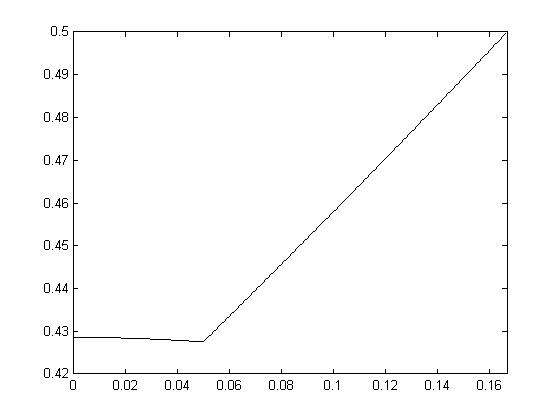
\includegraphics[height=3in, width=4.25in]{unweight.jpg}
\end{center}
\caption{Government Welfare with Partially Weighted Objective Function \label{fig:unweight}}
\end{figure}

This result that government welfare is strictly increasing in the political pressure parameter would seem to be related to the fact that, although $\ga$ is often referred to as a ``political economy weight,'' Expression~\ref{eq:wel} is only partially weighted. That the extra importance given to profits of importers when $\ga$ increases is pure additional welfare with no concomitant reduction elsewhere may be an assumption worth weakening, particularly in the context of endogenous political activity. 

One alternative formulation for the government objective function is one in which $\ga$ is a true weight in the following straightforward sense:
\begin{equation}
  \frac{1}{4+\ga(e)}CS_X(\tau) + \frac{\ga(e)}{4+\ga(e)}PS_X(\tau) + \frac{1}{4+\ga(e)}CS_Y(\tau^*) + \frac{1}{4+\ga(e)}PS_Y(\tau^*) + \frac{1}{4+\ga(e)}TR(\tau)
  \label{eq:weighted}
\end{equation}

See the \hyperlink{sol_weighted}{Appendix} for the mathematical derivations corresponding to Figure~\ref{fig:weight}. They show that, particularly for the trade agreement tariffs, government welfare first declines and then increases, with the minimum value occurring around $\tau = 0.057$ and $\ga = 1.05$. The maximum still unquestionably occurs at the maximum value of $\ga$, which leads to the prohibitive tariff of $\frac{1}{6}$. But if a government's objective function is closer to Expression~\ref{eq:weighted} than Expression~\ref{eq:wel}, the government may be interested in using the trade agreement to manipulate the lobby's behavior and therefore the political pressure that it experiences.
	
\begin{figure}
\begin{center}
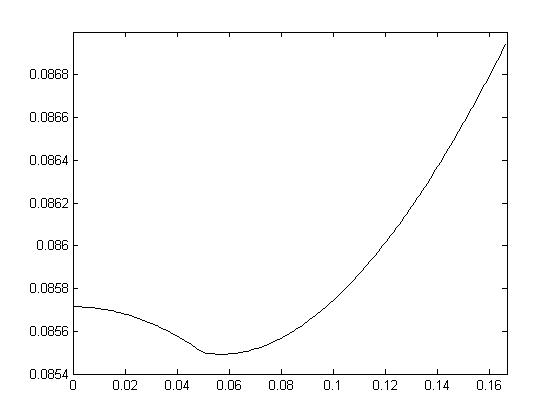
\includegraphics[height=3in, width=4.25in]{weight.jpg}
\end{center}
\caption{Government Welfare with Weighted Objective Function \label{fig:weight}}
\end{figure}

Whether or not the optimal trade agreement would set a tariff cap aimed at reducing lobbying depends on the lobby's incentives, which depends in turn on the shape of $\ga(e)$. Let's look at two parameterizations in a simple family of functions for $\ga(e)$ that demonstrate drastically different outcomes.

I begin with $\ga(e) = 1 + e^{.1}$. With no trade agreement, the lobby maximizes its net profits by choosing $e=0.0016$, which results in $\ga=1.525$ and a Nash tariff of $0.129$. Import-competing producer (net) profits are $0.1025$, while government welfare is $0.0862$. Because joint government welfare is convex in the tariff, the solution will be at a corner: either at $\tau^R_{W,e} =0$ or at the highest level for which the lobby will exert effort, i.e. the Nash tariff. Since joint welfare at the zero tariff is $0.0857$, the tariff cap is set at the trivial level of the non-cooperative Nash tariff. 

Here, given the way in which lobbying effort is translated into political support as represented by $\ga$, the government cannot improve its welfare by manipulating lobbying incentives. Discouraging lobbying would reduce welfare; in this parameter range, the government's interest is solely in encouraging lobbying effort, and there is nothing it can do in this regard.

%This is does through the introduction of the trade agreement: by making protection more expensive, on the margin the lobby pays more in order to get even less protection than it did in the absence of the agreement. But there is nothing further the government can do to increase $\ga$.

This example stands in contrast to one in which $\ga(e) = 1 + e^{.3}$. With no trade agreement, the lobby maximizes its net profits by choosing $e=0.0010$, which results in $\ga=1.126$ and a unilateral tariff of $0.068$. Import-competing producer (net) profits are $0.0921$, while government welfare is $0.0855$. Since joint government welfare is higher at free trade, the trade agreement will set the tariff cap at zero, profits decrease to $0.0816$, and government welfare increases to $0.0857$.

In this case, again the government does not have means to encourage any additional lobbying, but it can improve its situation by discouraging lobbying. By setting a tariff cap of zero---assuming the conditions for self enforcement outlined in Section~\ref{sec:selfweak} are met---the government can use the trade agreement to improve welfare by changing lobbying incentives and therefore the political pressure it encounters. The stark prediction that the best the government can do is to set the trade agreement to zero would be softened in an environment such as that in Section~\ref{sec:escape2} where there are both endogenous and exogenous sources of political pressure or with a government welfare function that has an interior global maximum in $\ga$. There are many candidate for the government objective function in which the maximum is strictly interior. For example, in \Textcite{ethier2012}, returns to lobbying decrease as tariffs increase. In the current model, one could take government welfare to be quadratic in $\ga$ or to simply subtract lobbying effort from Equation~\ref{eq:wel}. 

With the fully-weighted welfare function, we see that the trade agreement is employed to different ends depending on $\ga(e)$. If the lobby's ability to make an impact on the political process is strong enough, the government will be chiefly concerned with the profits of the import-competing industry and will use the trade agreement solely to internalize the terms-of-trade externality. However, if the lobby's impact is below a given threshold, the distortions that protection create are weighed more heavily and the government will use the trade agreement to rein in lobbying activity.

%In either case, we see that the government is able to provide reduced protection while extracting more effort from the lobby under a trade agreement: internalizing the terms of trade externality increases the marginal cost of protection.

I do not argue that the government welfare function in Expression~\ref{eq:weighted} perfectly represents the preferences of those who negotiate trade agreements. I only want to make the point that assumptions on the features of the government objective function can be important drivers of results on the role that trade agreements can play. 

Examining these alternatives in combination with endogenous lobbying points out that the idea that trade agreements can function as domestic political commitment devices may be more general than previously demonstrated. It can also provide a bridge between the theoretical literature and the claims of trade policy practitioners that an important role of trade agreements is to rein in protectionist pressure.

\subsection{Exogenous Political Pressure and Incentive Compatibility}
In order to compare the results for the case of endogenous political pressure to \Textcite{bs2005} results for exogenous political shocks, I provide the essentials of their setup. 

They assume that $\ga$ and $\ga^*$ are each drawn independently from probability distributions with cumulative distribution functions $H(\ga)$ with $h(\ga)=H'(\ga)$. The support for this probability distribution is $\left[\un{\ga}, \ov{\ga} \right]$ where $\ov{\ga} < \frac{7}{4}$. They also assume $\ga$ and $\ga^*$ are private information.

This leads to a concern about incentive compatibility. It must be in a government's best interest to truthfully reveal its $\ga$ or else it will misrepresent its private information about $\ga$ in order to raise tariffs and create a terms-of-trade gain, thereby improving its unilateral welfare. They provide conditions that guarantee incentive compatibility on page 481.

On a separate note, it is important to make clear that in this strand of the literature, it is assumed that trade agreements are negotiated to maximize the expected welfare of politically motivated governments given the exogenously-determined political pressure they expect to face at the time of the agreement's implementation. I will follow this convention throughout.




\section{Rigid Tariffs with Endogenous Political Pressure}
\label{sec:rigid}
We are now ready to demonstrate the implications of taking account of endogenous political pressure on some central design features of trade agreements. I develop some basic results about the design of trade agreements with tariff caps when political pressure is endogenous and compare and contrast these results to the case where political considerations are exogenous.

In Section~\ref{sec:escape2} I will examine the more realistic case where endogenous and exogenous political forces coexist. Until then, I will consider the cases separately to clearly establish the different dynamics that arise from the two distinct types of influence. I begin with the case of rigid tariffs---that is, trade agreements that have no provision for flexibility. Rigid tariffs cannot be made to depend on the realized level of $\ga$ and so incentive compatibility considerations do not come into play.

Because the trade agreement is set ex-ante---that is, before political pressure is realized, regardless of its source---the process of choosing the optimal tariffs differs across the two cases. When $\ga$ is exogenous, the government must plan for level of $\ga$ it will face \textit{in expectation}. When political pressure in purely endogenous, the government has perfect foresight to plan for the $\ga$ it will face but must confront the fact that its decisions affect lobbying incentives.

With the introduction of endogenous political pressure, one must take a stand on whether lobbies influence the formation of the trade agreement or are only active once the trade agreement is in place. Since a central goal here is to determine the impact of relaxing the assumption that political pressure is exogenously determined, I assume the latter to make the comparison most direct to this literature in which by definition there can be no endogenous political pressure at the trade agreement formation stage. The former, which is undoubtedly an important possibility in many institutional settings, is left as an important extension.\footnote{Note that the endogenous trade policy literature that involves trade agreements (e.g. \Textcite{gh95}, \Textcite{mrc2007}) explicitly assumes that trade agreements are formed in the face of political pressure while answering a different set of questions. Results for the case of ex-ante lobbying are available from the author upon request.}


\subsection{Perfect External Enforcement}
\label{sec:perfect}
I begin by assuming that perfect external enforcement is available for ensuring that the trading partners abide by the terms of the trade agreement. Although this is an unrealistic assumption, it establishes an important baseline case. Section~\ref{sec:self} adds the requirement that trade agreements be self-enforcing.

I restrict attention to the case of weak bindings throughout as this is the more interesting and realistic case.\footnote{There \textit{is} an extreme difference in outcome for strong bindings between exogenous and endogenous cases. When the terms of the agreement are that tariffs must be set at the precise value stipulated, the lobby has no incentive to exert effort and the trade agreement tariff is set at zero. Results are available upon request from the author.} Weak bindings are commonly referred to as tariff caps. When bindings are weak, the applied tariff can take any value as long as it is no greater than that which is agreed upon.

When political pressure is endogenous, in place of taking expectations over a range of probabilistically-determined levels of exogenous political pressure, we backward induct to determine the lobby's effort decision and the government's optimal choice of tariff caps in anticipation of the lobby's behavior.

In the final stage, the government will seek to maximize its welfare by choice of $\tau$ given the political pressure that it faces and the enforcement of the tariff cap, here denoted $\tau_e^R$ for the case of endogenous political pressure with rigid bindings, as distinct from $\tau^R$ in the case of exogenous political pressure with rigid bindings. The home government unilaterally maximizes Expression~\ref{eq:wel} so that the applied tariff is the Nash tariff $\tau^N(\ga(e))$ as long as $\tau^N(\ga(e)) \leq \tau_e^R$. Otherwise, the government must set $\tau = \tau_e^R$ since the weak binding $\tau_e^R$ is externally enforced.

Knowing how the government will set the applied tariff, in the second stage the lobby makes its effort decision to maximize net profits according to Expression~\ref{eq:lv3}. If the lobby's optimal effort level in the unconstrained problem (label it $e^L$) would lead to $\tau^N(\ga(e)) > \tau_e^R$, the lobby will reduce its choice so that no effort is wasted. I label the lobbying effort choice that leads to the weak binding level as $e^R$ so that $\tau^N(\ga(e^R)) = \tau_e^R$. The lobby will choose $e^R$ when its optimal effort would lead to a tariff level higher than that allowed by the weak binding; otherwise it will choose its unconstrained optimal effort $e^L$. 

We are now in a position to determine how the governments set trade agreement tariffs. Their goal is to maximize their joint welfare as in Expression~\ref{eq:jv} given the behavior they expect from the lobbies. Again, we can restrict attention to the home country and the $X$ sector because of the symmetry and separability of the economy.

I assume for simplicity of exposition that the government does not set the tariff binding $\tau_e^R$ higher than that which would result from the lobby's optimal effort $e^L$, as setting a higher tariff cap would not change lobbying behavior or outcomes in any way.\footnote{The government's tariff cap choice can reduce lobbying effort; it cannot, however, increase lobbying effort above $e^L$. The government is unable to use a weak binding to encourage extra lobbying when only import-competing interests are represented by a lobby. Introducing lobbies for the export industry could reverse this: lobbying effort by exporters could be encouraged in support of capping the import tariffs of the partner country.}

This is in contrast to the case of exogenous political pressure, for which \Textcite{bs2005} show several interesting results.\footnote{Note that in their treatment, Bagwell and Staiger (2005) assume linear supply and demand.} In particular, they find that when governments negotiate commitments that take the form of weak bindings, the tariff caps they choose imply that applied tariffs will be set strictly below the bound level when governments experience low realizations of political pressure.

To understand how the optimal home tariff $\tau_e^R$ under the trade agreement is set, notice that it must maximize joint government welfare. As argued in Section~\ref{sec:nasheff}, joint government welfare (with variables that do not affect the $X$ sector suppressed) is
  \begin{equation}
		W_x \left(\ga(e),\tau) \right) + W_x^*\left(\tau \right)
	  \label{exp:1}
	\end{equation}
where the lobby will exert no more effort than that which produces the capped $\tau_e^R=\tau^N(\ga(e^R))$. Recall that the Nash tariff, $\tau^N(\ga(e))$ is the solution to the unilateral optimization problem the home government faces when choosing the applied tariff level in the final stage of the game. It is given by Expression~\ref{eq:nash}, which contains the mapping between the political pressure the lobby exerts and the government's unilateral tariff response. We can therefore use Expression~\ref{eq:nash} to determine the level of $e$ the lobby must exert in order to receive a particular $\tau^N(\ga(e^R))$ equal to the tariff cap $\tau_e^R$.

Ex-post lobbying will constrain the governments in that the $\ga\left(e^R\right)$ they experience will be determined through the unilateral maximization problem in the last stage. The governments get to choose the $\tau_e^R$ that maximizes their joint welfare, but they cannot change this future lobbying process; they can only reduce the level at which it takes place through the tariff cap.

Notice that the maximand in Expression~\ref{exp:1} is exactly the same as that in the third-stage maximization problem except it adds  foreign government welfare. This implies that $\tau_e^R$ is (weakly) lower than the unilateral tariff as the terms-of-trade externality is internalized.\footnote{The terms-of-trade motivation for the trade agreement may not strictly lower the tariff if the solution to the government's joint maximization problem is not interior in the sense that the governments want as much lobbying as possible. To illustrate: if joint welfare is everywhere increasing in $\ga$, although reducing tariffs would improve welfare when $\ga$ is \textit{exogenously given} because each country would not be imposing the terms-of-trade externality on the other, when $\ga$ is endogenous, reducing the tariff reduces $\ga$ and therefore joint welfare.\label{fn:tot}}

A second motive may be operative here that is absent in the case of exogenous political pressure. When the government's optimum in terms of $\ga(e)$ is lower than the lobby's, the government will use the trade agreement as a domestic political commitment device to manipulate ex-post lobbying incentives. Whenever the cap is strictly below the non-cooperative level, that is when $\tau_e^R < \tau^N$, the weak binding restrains political pressure.

On the other hand, if the level of the optimal weak binding $\tau_e^R$ is strictly positive, the weak binding is at least in part serving to generate political effort---most often thought of as campaign contributions---that the government finds beneficial from its politically-motivated point of view. The government could have chosen a cap of zero and eliminated lobbying activity altogether. In fact, any strong binding accomplishes this very feat, but is also \textit{unable} to generate lobbying activity because of its effect on lobbying incentives. Thus the introduction of endogenous political pressure provides an explanation of the prevalence of tariff caps: they are a a sort of carrot to encourage political contributions, or perhaps they should be seen as a stick with which to threaten the removal of protection if political support does not continue.

\begin{proposition}
    When political pressure is entirely endogenous and governments negotiate commitments that take the form of weak bindings, they will not set applied tariffs strictly below the bound level. Governments may use the weak tariff binding to restrain and/or encourage endogenous political pressure.
		\label{res:weak}
\end{proposition}

Thus we see that the governments can use a tariff cap to manipulate lobbying incentives so that political effort is neither too low or too high. Note that this is related to a point made by \Textcite{mrc2007}; in their model, tariff caps and exact tariff commitments are equivalent when factors are perfectly immobile as in this model.
					
	
\subsection{Self-Enforcing Trade Agreements}
\label{sec:self}
Here I remove the assumption of perfect external enforcement since external enforcement is not widely available in the context of international trade relations. External enforcement is replaced with promises of future cooperation and punishment is modeled via a repeated game. I begin by describing the repeated-game set-up. 

\subsubsection{Repeated Game}
Because the governments are faced with asymmetric information, perfect public equilibrium (PPE) is the appropriate solution concept. Here attention is restricted to symmetric, stationary PPE.
	
In order to establish an equilibrium, we must ensure that both the on-schedule (static) incentive constraint and the off-schedule (repeated-game) incentive constraint is satisfied. The former is trivially satisfied for the case of rigid bindings, so it is only the repeated-game constraint that must be considered here. Following most of the literature, I assume that any deviation triggers a reversion to the static Nash equilibrium---what is known as `grim trigger.'\footnote{See \Textcite{krw} for an alternative that takes seriously the threat of governments renegotiating out of punishments that are not themselves incentive compatible.\label{fn:krw}}
	%see KRW, Buzard 2014 for alternatives
	
\subsubsection{Self Enforcement}
\label{sec:selfweak}
When political pressure is exogenous, \Textcite{bs2005} perform a standard repeated-game prisoner's dilemma analysis and show that if governments are patient enough ($\de$ is sufficiently high), the optimal weak binding from the perfect external enforcement setting can always be sustained with repeated-game incentives.

When $\ga$ is endogenously-determined, repeated-game enforcement is altered relative to the case of exogenously-given political pressure. This is because, in place of a stochastic process that determines $\ga$, $\ga$ is determined by a new repeated-game player who cares whether the trade agreement is followed or reversion to the non-cooperative Nash outcome takes place.

Recall that the government's most preferred trade agreement tariff in this setting is the one that would allow it to provide the level of protection that is demanded \textit{ex-post}. Enforcement considerations do not change the protection demands when $\ga$ is exogenous. Similarly, because the government's objective function does not change and it is able to use the tariff cap to control the lobby's effort level, as long as the government is sufficiently patient, it would like to set the same tariff cap in the face of self-enforcement constraints as when the agreement is externally enforced.

When $\ga$ is exogenous, the optimal trade agreement tariff is the same under perfect external enforcement and self-enforcement because the change in enforcement conditions cannot affect the realization of $\ga$. In contrast, moving from a static problem with external enforcement to a repeated-game problem with an enforcement constraint changes the lobby's decision problem. Moving to the repeated-game environment with self enforcement does not alter the government's ideal trade agreement tariff, but the introduction of the lobby creates the possibility that the politically-optimal trade agreement tariff may not be self-enforcing.

Let us see how this works. Again, because of symmetry and separability, we can focus on the home government's choice of $\tau$ and the $X$ industry.

The government's incentive constraint is given by
  \begin{multline}
    \frac{\de}{1-\de} \left\{W_X(\ga(e^R),\tau_e^R) + W_X^*(\tau_e^R) - \left[W_X(\ga(e^N),\tau^N(\ga(e^N)) + W_X^*(\tau^N(\ga(e^N)) \right] \right\} \\ \geq W_X(\ga(e^B),\tau^B(\ga(e^B)) - W_X(\ga(e^R),\tau_e^R)
		\label{exp:govincent}
  \end{multline}
where $\de$ is the discount factor assumed common to the government and lobby, $\tau_e^R$ is the same tariff cap from Section~\ref{sec:perfect}, and $\tau^B$ is the ``break'' tariff. Any $\tau > \tau_e^R$ is sufficient to breach the trade agreement and trigger Nash reversion; $\tau^B(\ga(e^B))$ is defined as the tariff the government would choose as unilaterally optimal if faced with $e^B$, where $e^B$ is the minimum lobbying effort that would give the government incentive to break the trade agreement in the absence of external enforcement.

On the left side of the inequality is the discounted gain from maintaining the trade agreement relative to Nash reversion. In order for the government to have the incentive to abide by the agreement, this must be at least as large as the benefit to cheating. This is the current period increase in unilateral welfare from the tariff applied when breaking the agreement and is given on the righthand side of Inequality~\ref{exp:govincent}.

For a given $\de$, $\tau^B$ and $e^B$ are derived using Equation~\ref{eq:nash} and Expression~\ref{exp:govincent} evaluated at equality. $e^B$ can be interpreted as the minimum level of lobbying effort that will persuade the government to abrogate the agreement. It must provide significantly more unilateral welfare than the trade agreement tariff in order to compensate the government for the loss of cooperation in every future period.

The lobby's incentives must also be satisfied, as the government's decision on whether to abide by the agreement or break it depends on the amount of lobbying effort it encounters. In order for the lobby to prefer the trade agreement tariff to the option of causing the agreement to be broken and tariffs to revert to the non-cooperative level, the following must hold
\begin{equation}
  \frac{1}{1-\de}\left[\pi(\tau_e^R) - e^R\right] \geq \pi(\tau^B) - e^B + \frac{\de}{1-\de}\left[\pi(\tau^N) - e^N\right]
	\label{exp:lobby}
\end{equation}
That is, the present discounted value of net profits under the trade agreement must be weakly higher than one period of net profits from the ``cheater'' tariffs and the discounted future Nash profits.

Here we have the possibility of a starkly different result from that under exogenous political pressure. Instead, the addition of a second incentive constraint can make it impossible to sustain the politically efficient tariffs.

To see this, start by noticing that the lefthand side of Expression~\ref{exp:govincent} is increasing in $\de$, while the righthand side is constant in $\de$. That is, as the government becomes more patient, it is easier to satisfy the government's constraint. Equivalently, it requires a larger $e^B$ to violate the constraint.

Shifting attention to the lobby's incentive constraint in Expression~\ref{exp:lobby}, this becomes harder to satisfy as $\de$ increases for most levels of the trade agreement tariff. That is, the lefthand side is decreasing and the righthand side is increasing as a direct function of $\de$. When taking into account the influence of $\de$ from the government's constraint on $e^B$, for a small part of the parameter space where $e^B$ must be very large, it's possible for the lobby's constraint to eventually loosen as $\de$ increases since $\pi(\tau^B) - e^B$ decreases to the right of $\tau^N$.

In general, however, we cannot be guaranteed that even the most patient government can sustain cooperation at the politically optimal trade agreement level. At issue is the behavior of the lobby, which is now a formal player in its own right and must be incentivized to keep its behavior on the equilibrium path. More patient lobbies are willing to work harder to encourage the government to break the trade agreement so that they can enjoy infinite periods of Nash tariffs. Increasing the discount factor makes it more difficult rather than easier to satisfy the lobby's constraint.\footnote{The essential point underlying this result was first made by \Textcite{buzard2013a}.}

\begin{proposition}
  The presence of the lobby as a repeated-game player may imply that the politically optimal self-enforcing trade agreement tariff is strictly greater than $\tau_e^R$.
	\label{res:repeated}
\end{proposition}

If there is no $\de$ such that Inequalities~\ref{exp:govincent} and \ref{exp:lobby} hold simultaneously, the governments must raise the trade agreement tariff, which loosens both incentive constraints simultaneously.

\section{Endogenous Political Pressure and the Escape Clause}
\label{sec:escape}
I begin by following \Textcite{bs2005} in examining a trade agreement with an escape clause by adding a second negotiated binding to the agreement so that there is one (weak) binding for when political pressure is low and a higher, weak binding for exceptional circumstances of high levels of political pressure. Escape clauses are common features of trade agreements in practice, and when one models political pressure as exogenous, an escape clause seems attractive: in the presence of a particularly large negative political shock, being bound to a tariff designed for normal times would cause significant welfare losses to the politician.

However, because the tariff allowed under the trade agreement with an escape clause varies with the announced level of political pressure, the incentive compatibility constraint now comes into play: a government may gain an advantage by misreporting the level of $\ga$ it experiences. In their Proposition 4, Bagwell and Staiger show that a trade agreement with a costless escape clause cannot improve welfare because it cannot be made incentive compatible. No matter the realization of the stochastic $\ga$, it is always in the government's interest to announce that $\ga$ is high, which allows it to apply any tariff up to the higher weak binding. This deviation improves unilateral welfare while imposing a terms-of-trade externality on the trading partner.

A similar problem arises in the case of endogenous political pressure, but with no parallel potential gain. The problem of asymmetric information remains, as lobbying effort is not observable to the trading partner. The appeal of an escape clause is to provide the flexibility of a higher binding in exceptional circumstances when political pressure is randomly high. But in the stark case under examination here with purely endogenous politics, an exceptionally high $\ga$ can only derive from higher effort exerted by the lobby. If one chooses an optimal tariff cap, a second, higher cap can only encourage excess, sub-optimal lobbying.

Thus, while with a costless escape clause there is no way to make truth-telling incentive compatible, this is of little consequence. The government would actually be \textit{truthfully} reporting the higher level of $\ga(e)$ as long as it is worthwhile for the lobby to increase its effort to this level. The appeal of an escape clause is missing in this case. What remains is the potential for governments to be forced ex-post to exploit the escape clause in a way that damages their ex-ante welfare.\footnote{Notice that the ex-post rent-seeking that creates this ex-ante loss is different in the two cases. With exogenous shocks, the government increases its welfare through the terms-of-trade channel. With endogenous political pressure, the lobby extracts the rents.}

\subsection{Escape Clauses with Strong Bindings}
\label{sec:strong}
Suppose that political pressure derives only from endogenous sources but an escape clause is to be implemented anyway. As \Textcite{bs2005} point out, in order for an escape clause to be useful to the government, it should be costly so that its use can be made incentive compatible. They suggest several avenues for introducing a cost for the use of the escape clause.

One possibility is to make the escape clause tariff a strong binding instead of a weak binding. The cost imposed here is the following: if the realization of $\ga$ is such that the optimal tariff is above the agreed-upon weak binding for normal times but below the strong binding for exceptionally high realizations of political pressure, the government must choose between applying the lower weak binding and the precise escape-clause tariff. In this case, there are welfare losses from implementing a sub-optimal tariff level that are not present if the escape clause tariff is a weak binding.

When $\ga$ is endogenous, the government is not subject to such random, unpredictable realizations of political pressure. It can avoid such costs by setting the escape clause tariff precisely at the level the lobby will find optimal to ask for; it thus avoids the mechanism that allows for incentive compatibility as well. In addition, given that the lower, normal binding could be set optimally for the government, the government only stands to lose from entering into a trade agreement with such an escape clause. This is, again, assuming that there is no exogenous source of political shocks for which flexibility is desired.

Thus, in this case the strong binding does not really create an incentive-compatibility-inducing cost, but again the central problem is that of lobbying incentives. This could explain, as Bagwell and Staiger point out, why the WTO does not incorporate strong bindings for the escape clause.

\subsection{Escape Clauses with Side Payments}
Suppose instead that the use of the escape clause must be accompanied by a side payment when the higher tariff is applied. In efficiency terms, this will only redistribute surplus from the trading partner who invokes the escape clause to the partner whose goods are targeted by the higher tariff. This is not entirely realistic as cash transfers are rarely observed in the WTO and other trade agreements; instead compensation is in the form of retaliatory tariffs---which are not efficient.\footnote{Note also that the WTO Safeguards agreement has a dynamic use constraint but removes the requirement for compensatory action in the first three years.}

\Textcite{bs2005} show that, again, the transfer function must satisfy two incentive compatibility conditions: the static condition that makes it worthwhile to truthfully reveal one's true $\ga$, and the repeated-game incentive constraint required for self-enforcement. Given these requirements, their Proposition 5 establishes that an appropriate transfer scheme can make a trade agreement with an escape clause incentive compatible.

Given the limited nature of the result in Section~\ref{sec:selfweak}, for the case of endogenous $\ga$ I restrict attention to economies in which the jointly optimal weak binding is supportable. The conditions given in Lemma 1 of \Textcite{bs2005} are not materially changed by substituting endogenous $\ga$ for exogenous $\ga$, so incentive compatibility in the static sense is ensured.

It is the repeated-game, or off-schedule, constraint that is significantly altered. The new element compared to self-enforcement without the escape clause is that the government can cheat on both its tariff and its transfer payment. With no lobby, the Bagwell and Staiger result shows that this temptation can be overcome; the question is whether the lobby makes this more difficult.

The answer is that it does not. Assuming the lobby represents a negligible share of the population, it does not bear the cost of the transfer. In fact, because it receives all the benefit of the tariff increase under the escape clause with none of the burden of paying for it, the lobby is much better off under the trade agreement with escape than the trade agreement without escape.

%	\item BUT need to check equilibrium impact on lobby's utility--does something in this constraint make it cheaper / more expensive for lobby to get the tariff it wants?

Here, we have a mechanism that is incentive compatible despite the presence of lobbying. It makes the lobby exert effort in order to receive the higher level of protection under the escape clause just as in the other mechanism. And although the burden of the transfer falls on others in the economy, at least the trading partner is compensated. Here the government is truthfully revealing the level of political pressure it faces, but that pressure is created by endogenous forces that are intensified by the existence of the escape clause. The escape clause is incentive compatible, but as will be clarified in the next section, the spirit of the escape clause is not necessarily upheld.

In the next section, I turn to the implications for the structure of the WTO procedures for administered protection, and the escape clause in particular, in a more realistic setting where both exogenous political shocks and endogenous lobbying are present.


\subsection{Escape Clauses with both Exogenous and Endogenous Political Pressure}
\label{sec:escape2}
When $\ga$ is exogenous, the purpose of the escape clause is clear: it improves welfare by allowing the government to apply a higher tariff when the realization of $\ga$ is particularly high. In this case, the government would suffer significant welfare losses from abiding by the lower, normal tariff binding, and may find its interests are better served by abrogating the trade agreement if no escape were permitted.

There is no such benefit when political pressure is purely endogenous. All political pressure can be anticipated by the government and accounted for in the normal binding, so any higher tariff provided for escape would either not be used or would reduce government welfare by encouraging excess political pressure in the case where the trade agreement tariff is being employed to reduce lobbying.

In reality, it is likely that both exogenous shocks and endogenous forces contribute to the pressure to which policy makers are subject. Thus, the need for flexibility that derives from the purely exogenous case remains and we desire to see if it is possible to implement an escape clause in the face of the additional endogenous source of political pressure.

So we go back to the general formulation where $\ga$ is a function of both lobbying effort $e$ and exogenously-determined events $s$ that create political pressure as in \Textcite{ms2011}. Let us take a simple case where the political pressure from the two sources are additively separable so that $\ga(s,e) = \ga(s) + \ga(e)$. Various interpretations are possible, including that some part of $\ga(s)$ derives from lobbying associated with the exogenous shock, while $\ga(e)$ is pure rent-seeking. Assume the interesting case that $\ga(\un{s}) < \ga(\ov{s}) < \ga(e^L)$; that is, the optimal political economy parameter from the lobby's point of view is greater than that which results from even the highest value of the exogenous shock variable. This implies that the lobby has the incentive for all realizations strictly below $\ov{s}$ to add pressure to that which comes directly from exogenous sources.

Imagine first that $s$ and its mapping $\ga(s)$ are completely unverifiable so as to make the analogy to the exogenous shocks examined above complete. There is a large parameter space over which an escape clause could not function in the way it is intended. When the realization of the shock is high, the government will report the high shock and apply the escape clause tariff. But when the shock is low, the lobby will exert effort so that the sum of $\ga(s)$ and $\ga(e)$ equals the high realization.

\begin{proposition}[Ineffectiveness of Political Criterion for Escape Clause]
    Assume $\ga(s,e)$ is additively separable in $s$ and $e$ with $s$ and $e$ independent. If an escape clause conditions on $\ga(s,e)$ and the lobby's preferred tariff is higher than the escape clause binding, the lower ``normal'' tariff binding will never be applied.
\end{proposition}

From the point of view of maximizing the political welfare of the governments, this is only problematic if, as demonstrated in Section~\ref{sec:objfcn}, the governments' ex-ante welfare is reduced by excess lobbying. However, the problem is not interesting if government welfare is everywhere increasing in lobbying effort because the lower binding will be set to the prohibitive tariff in this environment with no counter-lobbying by export groups.

Given that the intent of the escape clause is to provide flexibility for high realizations of $\ga(s)$, we see that the presence of endogenous lobbying can easily destroy its efficacy as the lower binding will never be used. The water in the escape clause will be filled in by endogenous political pressure.

This is not a problem of incentive compatibility. Similar to \Textcite{beshkar2010b}, it can be shown [formal result coming soon] that a dispute settlement body that provides an independent signal about the value of $\ga(s,e)$ on which the governments condition punishments for misreporting can make truth-telling incentive compatible. That is, a government will not over-report its political-economy pressure in order to impose a terms-of-trade externality on its trading partner. But this is of little consequence because the political-economy parameter will always take on its highest value.

Given the inability of achieving the first best in this environment, what can be done? Unless political pressure that comes from a shock can be distinguished from political pressure that is purely rent-seeking, there appears to be little hope that the two can be disentangled through the investigation of a body such as the WTO's DSB. In fact, in its rulings the DSB does not appear to take into account political conditions at all.

It seems plausible that this kind of dynamic is the reason that use of the WTO Safeguards are predicated on verifiable economic indicators--the $s$'s. This would appear to be the only way to prevent lobbies from exploiting the escape clause for uses for which it was not intended. However, once a shock has occurred, given that the DSB cannot distinguish between $\ga(s)$ and $\ga(e)$, determining the tariff that should be applied could only be done if (a) the DSB has the mapping $s \rightarrow \ga$ \textit{and} this strong form of separability holds. These conditions seem unlikely to be met in reality and we observe, again, that the DSB makes no attempt to determine the political parameter. Without this information, it thus can only certify the legitimacy of a Safeguard measure and perhaps the level of tariff that is necessary to counteract $s$. It cannot determine the correct level at which the Safeguard measure should be applied for the purposes of matching the applied tariff to the political pressure felt by the government.

In the next section, I turn to the kind of escape clause that is both implementable and able---at least in some cases---to address shocks without encouraging rent-seeking.

\subsection{An Escape Clause For Endogenous Politics}
\label{sec:ECendog}
In this world that is far from first best, I next demonstrate how a WTO-style escape clause can allow flexibility in the face of fundamental shocks $s$ while discouraging lobbyists from using the shock as cover for rent-seeking behavior. The timeline is as follows:
\begin{enumerate}
	\item The government sets the trade agreement tariff $\tau_e^F$ cooperatively. I assume this is a weak binding. The subscript $F$ denotes the environment with flexibility to deal with shocks.
	\item The exogenous shock $s$ is realized. Its level is assumed costlessly verifiable for simplicity.
	\item The lobby chooses its effort level $e^F$.
	\item The government chooses the applied tariff level from among $\tau_e^F$, $\tau(s)$ and $\tau^B(\ga(s,e^F))$.
\end{enumerate}
I take the higher, `escape' tariff $\tau(s)$ to be continuous. If the government applies $\tau_e^F$, implementation of the agreement goes on as before. Consistent with the WTO Agreement on Safeguards, the government can apply the tariff that is necessary to remedy the economic injury---not necessarily equal to the political injury---caused by the shock, $\tau(s)$, with no retaliation for three periods. If the government applies a tariff that is higher than either $\tau_e^F$ or $\tau(s)$, it will choose its myopic best response to the pressure it experiences. I label this tariff $\tau^B(\ga(s,e^F))$, where $e^F$ must be high enough to give the government incentive to break the trade agreement in the absence of external enforcement.

This is a violation of the trade agreement even in the presence of the safeguard and incurs retaliation. It is a violation of the agreement because the applied tariff level is higher than is needed to remedy the injury caused by the shock; the WTO Agreement on Safeguards instructs that ``A Member shall apply safeguard measures only to the extent necessary to prevent or remedy serious injury and to facilitate adjustment'' (Article 5.1).\footnote{The paragraph goes on to give even more clarification: ``If a quantitative restriction is used, such a measure shall  not reduce the quantity of imports below the level of a recent period which shall be the average of imports in the last three representative years for which statistics are available, unless clear justification is given that a different level is necessary to prevent or remedy serious injury.''}

To see how such a scheme works in the context of repeated-game enforcement, we look to the incentive constraints of the government and lobby. I follow \Textcite{buzard2013a} by using limited reversions to the stage-game Nash equilibrium outcome. For ease of analysis, I use a punishment length of two periods. This implies that a country would return to the agreement either after applying a valid escape clause for three years or after violating the agreement.

The government's incentive constraint is given by
  \begin{multline}
    \left[1+ \de +\de^2 \right] \left\{W_x(\ga(s,0),\tau(s)) + W_x^*(\tau_e^F) \right\} \geq \\ W_X(\ga(s,e^F),\tau^B(\ga(s,e^F)) + W_x^*(\tau_e^F) + \left[\de +\de^2 \right] \left\{W_X(\ga(s,e^N),\tau^N) + W_x^*(\tau^N) \right\}
		\label{exp:govincentEC}
  \end{multline}
Label $\ov{e}$ the level of $e^F$ that is just high enough to cause the government to throw the trading relationship into dispute. We use $\ov{e}$ in the lobby's constraint, in which the lobby optimally exerts no effort if the government applies the safeguard tariff $\tau(s)$:
\begin{equation}
  \left[1+ \de +\de^2 \right] \pi(\tau(s)) \geq \left[1+ \de +\de^2 \right] \left\{\pi(\tau(\ga(s,\ov{e})) - \ov{e} \right\}
	\label{exp:lobbyEC}
\end{equation}

Depending on the level of $s$ and the properties of $\ga(s,e)$, the government may choose to set the trade agreement tariff in the presence of an escape clause $\left(\tau_e^R\right)$ so that in some cases the lobby's incentive constraint is violated. This would lead to the legislature's constraint being violated as well, creating a dispute. 

One important outcome \textit{does not} occur in this environment: lobbies do not use the escape clause as cover for rent seeking. The government may use the escape clause to provide extra protection to compensate for a shock. This provides a looser incentive constraint than in the absence of the escape clause and improves self-enforceability of the agreement. Or the lobbies may still find it in their interest to exert effort to encourage the government to provide this higher level of protection $\tau(\ga(s,e^F))$. This will provoke a dispute, but the protection afforded by the higher tariff will not be hidden behind the escape clause. So an escape clause for the purposes of providing breathing room from exogenous shocks \textit{is} possible.

It still does not seem feasible to provide this flexibility at precisely the level that the shock impacts the government's preferences $\ga(s)$ if the WTO does not know the mapping from $s$ to $\ga$. What's more, this may provide an answer to why Safeguard measures have fallen out of use. If the real purpose is to provide an outlet for political pressure, I have demonstrated above that the current WTO-style Safeguards rules seem designed explicitly to discourage such rent-seeking behavior. Thus if other measures such as Anti-Dumping Duties are more susceptible to manipulation, it seems natural that lobbies' efforts would migrate there.

	

%\section{Ex-Ante Lobbying}
%\label{sec:exante}

%%\documentclass[12pt]{article}

%\addtolength{\textwidth}{1.4in}
%\addtolength{\oddsidemargin}{-.7in} %left margin
%\addtolength{\evensidemargin}{-.7in}
%\setlength{\textheight}{8.5in}
%\setlength{\topmargin}{0.0in}
%\setlength{\headsep}{0.0in}
%\setlength{\headheight}{0.0in}
%\setlength{\footskip}{.5in}
%\renewcommand{\baselinestretch}{1.0}
%\setlength{\parindent}{0pt}
%\linespread{1.1}

%\usepackage{amssymb, amsmath, amsthm, bm}
%\usepackage{graphicx,csquotes,verbatim}
%\usepackage[backend=biber,block=space,style=authoryear]{biblatex}
%\setlength{\bibitemsep}{\baselineskip}
%\usepackage[american]{babel}
%dell laptop
%\addbibresource{C:/Users/Kristy/Dropbox/Research/xBibs/tradeagreements.bib}
%\addbibresource{C:/Users/Kristy/Documents/Dropbox/Research/xBibs/tradeagreements.bib}
%\renewcommand{\newunitpunct}{,}
%\renewbibmacro{in:}{}


%\DeclareMathOperator*{\argmax}{arg\,max}
%\usepackage{xcolor}
%\hbadness=10000

%\newcommand{\ve}{\varepsilon}
%\newcommand{\ov}{\overline}
%\newcommand{\un}{\underline}
%\newcommand{\al}{\alpha}
%\newcommand{\expect}{\mathbb{E}}
%\newcommand{\ga}{\gamma}
%\newcommand{\Ga}{\Gamma}
%\newcommand{\de}{\delta}

%\begin{document}

In many situations, it is realistic to assume that, in addition to the ex-post lobbying examined throughout this text, lobbying also takes place before the trade agreement is signed to affect its terms. Sections~\ref{sec:rigid} and \ref{sec:objfcn} have shown that, although ex-post lobbying occurs after the trade agreement is signed in order to impact the level of the applied tariff, it alters the incentives of governments when they negotiate the trade agreement. Similarly, ex-ante lobbying is aimed directly at changing the level of the trade agreement tariff, but here lobbies only engage in this activity in order to alter what will be possible ex-post.

One of the main implications of the possibility of ex-ante lobbying is the addition of a new time at which the lobby may have to exert influence. As in Section~\ref{sec:strong}, when facing a trade agreement in which commitments take the form of strong bindings, the lobby's optimal ex-post effort choice is zero. However, when facing a tariff cap, protection will only be supplied at the ex-post stage if the lobby exerts effort. Thus, ex-ante lobbying adds a second time at which the lobby may have an incentive to exert effort in the case of a tariff cap; it introduces a first time at which the lobby may supply non-zero effort in the case of a strong binding.

For simplicity, here I consider ex-ante lobbying when political pressure is endogenous only, i.e. there is no exogenous, probabilistic influence on $\ga$. Since there is no possibility of ex-ante lobbying in the \Textcite{bs2005} framework this paper follows, it must be determined how ex-ante lobbying can best be integrated into the model.

The \Textcite{bs2005} framework posits that governments negotiate the trade agreement so that they will be able to set the applied tariff that best matches the political pressure they experience ex-post. In the case of endogenous political pressure, I argue that the governments will tune the trade agreement to deliver the amount of lobbying effort that is in their best interest ex-post. How does this change when lobbies can influence the terms of the trade agreement?

A lobby knows that the trade agreement will bind its future action, so exerting effort at the ex-ante stage only matters insofar as it improves ex-post profits net of both ex-ante and ex-post lobbying effort.

Looking at the policy-makers, with ex-post pressure only, the governments are completely forward looking: they set the trade agreement with a view toward maximizing expected joint ex-post welfare. In order for ex-ante lobbying to have an effect, it must be that governments also receive some utility from the setting of the trade agreement itself: perhaps they receive or lose political capital from various interested parties, and can be persuaded to forgo future benefits if ex-ante lobbying is strong enough to outweigh those future concerns. 

Thus I model the influence of ex-ante lobbying on the governments' tariff-setting behavior as operating through a threshold. Recall how the trade agreement tariff is determined under ex-post lobbying only. Because the trade agreement can act as a commitment device, the governments choose the tariff level $\tau^R_{\cdot,e}$, and implicitly ex-post effort $e^{EP}=e^R_{\cdot,e}$, to maximize their joint political welfare as in Equation~\ref{exp:1}, subject only to the constraint that $\ga$ will be realized according to the ex-post lobbying process.
		
As discussed in Section~\ref{sec:objfcn}, depending on how government welfare changes as political pressure increases, the governments may be looking ahead and manipulating ex-post lobbying incentives when there is only ex-post lobbying. When ex-ante lobbying is possible the governments may have to raise the trade agreement tariff above $\tau^R_{\cdot,e}$ in order to respond to that pressure.

This is modeled here with a simple cut-off. The trade agreement tariff cap will be set according to $\ga\left(e^{EA}\right)$ instead of at $\tau^R_{\cdot,e}$ if $\ga\left(e^{EA}\right)$ would lead to a higher trade agreement tariff. If, on the other hand, $\tau = \frac{4(\ga(e^{EA})-1)}{25-4\ga(e^{EA})} < \tau^R_{\cdot,e}$, the governments respond to the higher ex-post pressure and set $\tau^R_{\cdot,e}$.

Thus the governments lose some measure of control with ex-ante lobbying. If $e^{EA}$ is low enough, ex-ante lobbying has no impact. But if $e^{EA}$ is above the threshold, the trade agreement tariff is strictly greater than $\tau^R_{\cdot,e}$ and so joint government welfare will not be at its globally optimal level. The trade agreement the governments choose will be constrained by ex-ante pressure.

We will see that this change to the government's preferences has the impacts one would expect, at least in the case of weak bindings (tariff caps): net profits for the lobby (weakly) increase, and net political utility for the governments (weakly) decrease. We begin with the less clear-cut case of strong bindings.

\subsection{Strong Bindings}
Let us first look at how ex-ante lobbying impacts trade agreements that involve strong bindings, or exact tariff commitments. We know that when there is only ex-post lobbying, $e^{EP} =0$ and $\tau^{EP} = \tau^R_{S,e}$. Since ex-ante effort will be sunk ex-post, the ex-post stage of the game that includes ex-ante lobbying is identical to the game without ex-ante lobbying. In the case of exact tariff commitments, because $e^{EP} = 0 \ \forall e^{EA}$, the lobby does not consider the impact of ex-ante lobbying on the ex-post effort level.

This thus looks like a problem with no ex-post lobbying, but where there is perfect enforcement of the tariff commitment. This collapses to a simple problem of maximizing joint government welfare with $e=e^{EA}$, and the lobby maximizing profits net of ex-ante effort facing the joint maximization of the governments.

Without knowing how government welfare varies in $\ga$, we can't say for sure the effect on government welfare at the ex-ante stage. As with the example in Figure~\ref{fig:weight}, joint welfare could fall but could also rise. Ex-post political pressure will not match ex-ante political pressure: because of the incentives involved with strong bindings, the home government will experience $\ga(0)$ but be forced to apply the ex-ante tariff, so this is a welfare loss relative to the no ex-ante case at this stage.\footnote{This is a government welfare loss from exact tariff commitments that is not accounted for in \Textcite{mrc2007} because of their assumption that the government has no bargaining power. It seems to be closely related that, in their model,  exact tariff commitments and tariff caps are equivalent in the case of perfectly immobile capital. As will be shown below, that is not the case here.} There is a very clear gain for the lobby relative to the case where there is no ex-ante lobbying; it can avoid any loss by setting $e^{EA}=0$.
				
\subsection{Weak Bindings}
In the case of weak bindings, or tariff caps, the ex-post stage will also work as in the no-ex-ante-lobbying case, that is, as in Section~\ref{sec:weak}, again because ex-ante effort is sunk at the ex-post stage. To recap, when there is no ex-ante lobbying---or ex-ante-lobbying is less important than ex-post lobbying---the governments choose the $\tau^R_{W,e}$ that leads to the level of ex-post political pressure that maximizes ex-ante joint welfare
		\[
		  W(\ga(e^R_{W,e})),\tau^R_{W,e}) + W^*(\tau^R_{W,e})
		\]
		knowing that the home government will set the applied tariff in the third stage unilaterally (i.e. $\tau^N(\ga(e^R_{W,e})) = \frac{8\ga(e^R_{W,e}) - 5}{68 - 8 \ga(e^R_{W,e})} = \tau^R_{W,e}$).
						
What is different here is that the tariff cap could be set higher than this level because of the presence of ex-ante lobbying. The lobby chooses its ex-ante effort level $e^{EA}$ taking into account that the governments will set either the optimal ex-post tariff cap $\tau^R_{W,e}$ or a higher cap in ex-ante stage given the $e^{EA}$ with which it is confronted.

The lobby maximizes $\pi(\tau^E(e^{EA})) - e^{EA} - e^{EP}(e^{EA})$, with a first order condition of 
	\begin{equation}
	  \frac{\partial \pi}{\partial \tau} \frac{\partial \tau^E}{\partial \ga} \frac{\partial \ga}{\partial e^{EA}} = 1 +\frac{\partial e^{EP}}{\partial e^{EA}}
			\label{eq:ea}
	\end{equation}
This condition illustrates that, when it is operative, the governments choose the tariff cap according to Expression~\ref{exp:1} with $e^{EA}$, but the lobby still has to exert effort ex-post to receive the applied tariff. $e^{EP}$ is the amount the lobby pays according to Equation~\ref{eq:nash} to achieve $\tau^E(e^{EA})$ (see Equation~\ref{eq:eff}).

The lobby sets $e^{EA}$ according to this condition as long as 
	\begin{equation}
		\pi(\tau^E(e^{EA})) - e^{EA} - e^{EP}(e^{EA}) > \pi(\tau^N(e^R_{W,e})) - e^R_{W,e}.
		\label{ine:ea}
	\end{equation}
Otherwise, it maximizes net profits by setting $e^{EA} =0$.	

Thus if the lobby's incentives to exert pressure ex-ante are strong enough, they overpower the government's ability to use the trade agreement to directly manipulate lobbying incentives ex-post. The lobby can force the government to set a cap higher than the level that would optimize its welfare when there is no ex-ante lobbying. The lobby has no interest in a lower cap and can choose a zero effort level whenever positive effort would reduce its nets profits below the level with ex-post lobbying only. Therefore we have the following result:
		
\begin{proposition}
	When trade agreements take the form of weak bindings, the binding under ex-ante lobbying can only be (weakly) higher than when ex-ante lobbying is not possible. This can only (weakly) reduce the joint political welfare of the governments and it can only (weakly) increase net profits for the lobby.
\end{proposition}

\subsection{The Role of Trade Agreements with Ex-Ante Lobbying}				
To understand the function trade agreements serve in the presence of ex-ante lobbying when lobbying is endogenous, it is helpful to establish some facts about the levels at which tariff are set under various scenarios.

\begin{lemma}
  Trade agreements with ex-post lobbying lead to weakly lower tariffs (when bindings are either strong or weak) than those that are applied in the absence of an agreement.
	\label{lem:1}
\end{lemma}

See the \hyperlink{lem1}{Appendix} for the proof. Intuitively, both the terms-of-trade and domestic-commitment motives drive the governments to chose a (weakly) lower tariff than that which the home government chooses when there is no agreement.

It has been established above that the presence of ex-ante lobbying can only weakly increase tariffs from the ex-post agreement level with both strong and weak bindings. Lemma~\ref{lem:1} only establishes that the tariffs with ex-post lobbying are lower than the tariffs with no agreement; we would like to be able to derive a clear result comparing the tariff level with ex-ante lobbying to that with no agreement as well. Lemma~\ref{lem:2} does just that, but this is only possible in the case of weak bindings.

\begin{lemma}
  When bindings are weak, trade agreements with ex-ante lobbying lead to lower tariffs than those that are applied in the absence of an agreement. When bindings are strong, tariffs with ex-ante lobbying may be either higher or lower than those that are applied in the absence of an agreement.
	\label{lem:2}
\end{lemma}

See the \hyperlink{lem1}{Appendix} for the proof. The key insight here is that every unit of effort ex ante results in more political support than it would ex post because producer profits are counted the same while the terms of trade motivation is absent. With stronger incentives on the margin ex ante, we must rule out that the lobby exerts sufficiently more effort to overcome the internalization of the terms of trade externality that occurs through the trade agreement negotiation. The fact that the lobby must pay a second time, as well as from a lower base, is sufficient to mute its incentives at the ex-ante stage in the case of weak bindings; because it pays nothing at the ex-post stage with strong bindings, it is possible (although not likely) that the heightened incentives on the margin could lead to sufficient effort to produce a higher trade agreement tariff than that which the lobby would achieve with unilateral tariff setting. 

\begin{proposition}
	When trade agreements take the form of weak bindings and political pressure is endogenous, tariffs are always lower under trade agreements than in the absence of a trade agreement. 
\end{proposition}

This follows directly from Lemmas~\ref{lem:1} and \ref{lem:2}, since tariffs under ex-ante lobbying are set either in line with lobbying effort according to the first order condition (\ref{eq:ea}) or via ex-post incentives. Although Lemma~\ref{lem:2} shows that ex-ante effort will be strictly lower than effort under no trade agreement, it is possible that ex-ante effort will be nil and the trade agreement level will be set by ex-post incentives that provide for a tariff at the non-cooperative level (see Section~\ref{sec:objfcn} for an example).\footnote{Note that it is possible to have positive ex-ante lobbying when $e^R_{W,e}$ is restrictive, notably in the case where joint government welfare is concave in $\ga$ with a strict interior maximum. This implies that government welfare must eventually decrease in $\ga$, as in \Textcite{ethier2012} where there are diminishing returns to lobbying as tariffs increase. In the current model, one way this can arise is if $\ga$ is taken to be a decreasing function of $\tau$.}

A similar result clearly does not hold for strong bindings, and adds to the list of potential reasons why we do not see trade agreements take this form in reality.

This contrasts with \Textcite{mrc2007}. In their model, which also features endogenous political pressure with ex-ante lobbying, tariff caps and exact tariff commitments are equivalent in the case of perfectly immobile capital. This seems to be the result of their assumption, within the context of a cooperative bargaining solution for the trade agreement phase, that the lobby has all the bargaining power and thus receives all rents. Because the lobby receives protection ex post without exerting effort under exact tariff commitments, these two types of bindings lead to very different decisions ex-ante and splits of the surplus ex-post in the model under consideration here.\footnote{One reason the lobby is not included in the cooperative bargaining formulation here is that it leads to the strange outcome that the governments overweight the lobby's profits even when the lobby exerts no effort ex ante.}

Focusing on the case of weak bindings (i.e. tariff caps), we see that, as long as governments want to restrain lobbying, relative to non-cooperative levels, trade agreements will deliver this result even when ex-ante lobbying is possible. If a government wants to encourage political pressure, it may want to consider eschewing trade agreements, although the tradeoff is losing the ability to internalize the terms of trade externality. If a government wants to restrain political pressure, a trade agreement is doubly good.

There are several avenues through which trade agreements mute lobbying incentives. First, according to Condition~\ref{ine:ea}, ex-ante lobbying may be too costly since it adds a second time at which the lobby has to exert effort. When the lobby does find it advantageous to participate in ex-ante lobbying, although on the margin the incentives are stronger, the same effort produces a lower trade agreement tariff ex-ante than ex-post because $\ga$ is translated via Equation~\ref{eq:eff} instead of Equation~\ref{eq:nash} as when there is only ex-post lobbying. Thus not only must the lobby exert effort a second time, but it must work harder for the same level of protection ex-ante.

This points out an important role of trade agreements vis-\`{a}-vis political pressure groups: relative to ex-post lobbying, ex-ante lobbying gives them more ability to exert influence, but at a significantly higher cost. If either that higher cost or some institutional constraint makes only ex-post lobbying feasible, the governments can use the trade agreement to exert more significant control over the trade policy outcome.

%\end{document}

\section{Conclusion}
\label{sec:concl}
I have shown that accounting for endogenous lobbying has important implications for the design of trade agreements. For instance, tariff caps may be used alternatively to reduce lobbying activity, or to incentivize lobbies to remain active after a trade agreement is in place.

The addition of the lobby can make it harder to sustain cooperation and complicates the incentive compatibility problem associated with the use of escape clauses. The temptation for lobbies to exploit the opportunity presented by an escape clause provides a justification for the WTO requirements that verifiable economic conditions are met in order to legally invoke these protections.

I introduce a fully-weighted government utility function that is a slight modification of the standard Baldwin-style government objective function to demonstrate that it may be in even a politically-motivated government's interest to use a trade agreement to restrain political activity. The fact that the WTO Safeguards Agreement replaced compensation in the first three years of the invocation of a safeguard with a dynamic use constraint is consistent with the idea that the organization and the governments that constitute it are working to reduce rent seeking by lobbies. Section~\ref{sec:escape} demonstrates that lobbies do not care about the compensation since the costs do not fall on them, whereas a dynamic use constraint directly affects their ability to receive protection in the future.

There are many exciting avenues to extend this work. This simple framework demonstrates a tractable way to introduce endogenous political pressure into many of the important questions that have been and are currently being explored concerning the design of trade agreements and the institutions that facilitate them.

%The discussion in Section~\ref{sec:exante} presumes both that there are no significant interactions between lobbies and that governments are free to choose which sectors are part of a trade agreement, but these decisions are part of a more complicated game that is, in particular, influenced by WTO rules.

Taking into account the interactions between multiple lobbies, the influence of WTO rules, and differences in the $\ga$ functions across industries---that is, in how political pressure translates into weight in the policy-making process---seems like an important and interesting avenues for further study.

In particular, here there is no scope for the government to encourage lobbying above the level that is optimal from the special interest group's point of view; adding additional lobbies may create insights to this effect. There is also strong potential to gain insights concerning very realistic dynamics between political and economics shocks and lobbying, especially insofar as they impact questions of enforcement and administered protection.

As in \Textcite{zissimos}, it would also be interesting to compare the Nash-reversion punishment to punishment via 'withdrawal of equivalent concessions,' as it appears on the face of it that this environment may provide a justification its use. The intuition is the following: \Textcite{buzard2013a} shows that the lobbying effort required to cause the government to enter into a dispute is higher than the Nash equilibrium effort levels. Then the tariffs during a dispute are also higher, and punishment at this higher level would be more severe than Nash---both for the government and the lobby.\footnote{\Textcite{beshkar2010a} shows that when one assumes that utility is not transferable between countries as has become common in the literature, the optimal mechanism involves less-than-proportional retaliation against parties who have defected from the agreement. \Textcite{martinvergote} demonstrate that future punishment provides for higher welfare than contemporaneous punishment when governments are sufficiently patient. Indeed, they show that retaliation is a necessary feature of any efficient equilibrium in this environment. \Textcite{hungerford} and \Textcite{riezman1991} also consider the impact of different assumptions about reactions and timing of punishments for deviations from agreements.}


\section{Appendix}
\noindent \textbf{\hypertarget{envelope}{Unilateral and Joint Welfare Maximized at same $\ga$}}: \\
Starting with the non-cooperative maximization problem with respect to $\ga$:
\[
 \max_{\ga} W_x(\ga,\tau) + W_y(\tau^*)
\]
The first order condition is
\[
	\frac{\partial W_x}{\partial \ga} + \frac{\partial W_x}{\partial \tau}\frac{\partial \tau}{\partial \ga} = 0
\]
In an envelope-theorem style result, because the Nash tariff is the result of the government's optimization with respect to $\tau$, $\frac{\partial W_x}{\partial \tau}=0$ so that the first order condition reduces to $\frac{\partial W_x}{\partial \ga} = 0$.
				
Turning to the maximization of joint welfare in the trade agreement, we have
\[
  \max_{\ga} W_x(\ga,\tau) + W_y(\tau^*) + W_x^*(\tau)+ W_y^*(\tau^*)
\]
The first order condition is 
\[
  \frac{\partial W_x}{\partial \ga} + \frac{\partial W_x}{\partial \tau}\frac{\partial \tau}{\partial \ga} + \frac{\partial W_x^*}{\partial \tau}\frac{\partial \tau}{\partial \ga} = \frac{\partial W_x}{\partial \ga} + \left[ \frac{\partial W_x}{\partial \tau} + \frac{\partial W_x^*}{\partial \tau}\right]\frac{\partial \tau}{\partial \ga} = 0
\]
Here, it is the efficient joint tariff that is chosen, and it is chosen precisely by setting the term in brackets equal to zero so that we have the first order condition simplifying to the same expression as in the unilateral case. $\hfill\blacksquare$


\vskip.3in
\noindent \textbf{\hypertarget{sol_weighted}{Optimal $\ga$ for Weighted Government Welfare Function}}: \\
The first order condition for the weighted welfare function in Expression~\ref{eq:weighted}
			  \[
				  \frac{\partial W}{\partial \ga} = \frac{1}{\left(4+\ga(e)\right)^2}\left[ - CS_X + 4 \cdot PS_X - CS_Y - PS_Y - TR \right] = 0
				\]
Examining the expression in brackets:				
				\[
				  - CS_X + 4 \cdot PS_X - CS_Y - PS_Y - TR = 
				\]
				\[
				  -\frac{9-24\tau + 16\tau^2}{98} + 4\frac{4+8\tau + 4\tau^2}{49} - \frac{7\tau - 42\tau^2}{49} - \frac{9+18\tau + 9\tau^2}{98} - \frac{16-24\tau + 9\tau^2}{98}
				\]
				\[
				  = \frac{-9 + 32 -9 -16}{98} + \frac{24 + 64 -14 -18 +24}{98} \tau + \frac{-16 + 32 + 84 - 9 - 9}{98}\tau^2
				\]
				\[
				  = \frac{-2}{98} + \frac{80}{98} \tau + \frac{82}{98}\tau^2
				\]
			This expression is negative at $\tau=0$ and increases monotonically with an interior minimum; note the second derivative is strictly positive.
				
				Because $\tau$ is an increasing function of $\ga$, this pattern holds for $\ga$ as well. $\frac{1}{\left(4+\ga(e)\right)^2}$ is positive (and decreasing as a function of $\ga$), so the pattern holds for the derivative as a whole. Thus the FOC delivers a minimum point and the maximum must be at one of the endpoints. Calculations show that $W(\ga=1.75) > W(\ga=1)$. $\hfill\blacksquare$

\begin{comment}
\vskip.2in
\noindent \textbf{\hypertarget{lem1}{Proof of Lemma~\ref{lem:1}}}: \\
In the case of strong bindings, this is immediate from Proposition~\ref{res:strong}. In the case of weak bindings, first examine the first order condition for unilateral tariff setting:
\[
  \frac{\partial W_X(\ga,\tau)}{\partial \tau} = - \frac{5}{49} - \frac{68}{49}\tau +\frac{1}{98}\ga\left[ 16 + 16\tau \right] = 0
\]
Substituting in the inverse of the solution function $\tau^N(\ga) = \frac{8\ga-5}{68-8\ga}$ for $\ga$, this is
\[
  \frac{\partial W_X(\ga,\tau)}{\partial \tau} = - \frac{5}{49} - \frac{68}{49}\tau +\frac{1}{98} \frac{68\tau+5}{8+8\tau} \left[ 16 + 16\tau \right] = 0
\]
This same solution for $\ga$ will be substituted into the first order condition for the joint maximization problem in the ex-post trade agreement game; the only difference is the foreign welfare $W_X^*(\tau) = \frac{25}{98} - \frac{3}{49}\tau + \frac{9}{49}(\tau)^2$ is added to the objective function. The derivative with respect to $\tau$, $- \frac{3}{49} + \frac{18}{49}\tau$ is strictly negative for all non-prohibitive levels of the tariff ($\tau \in \left[0,1/6\right)$) and 0 at the prohibitive tariff. Thus the first order condition for the joint problem is negative at the unilateral tariff; a (weakly) lower tariff must be chosen to achieve the maximal value of this objective function. As demonstrated in Section{sec:objfcn}, the domestic commitment motive may also drive the solution to the free trade corner solution. $\hfill\blacksquare$

\vskip.2in
\noindent \textbf{\hypertarget{lem2}{Proof of Lemma~\ref{lem:2}}}: \\
Denote the tariff with no agreement as $\tau^N(e^N)$. The lobby's effort level in the absence of a trade agreement is determined by the first order condition
	\begin{equation}
		\frac{\partial \pi}{\partial \tau} \frac{\partial \tau^N}{\partial \ga} \frac{\partial \ga}{\partial e^N} = 1
			\label{eq:nta}
	\end{equation}
In order to compare this with Equation (\ref{eq:ea}) for weak bindings, note that
  \[
	  \frac{\partial e^{EP}}{\partial e^{EA}} = \frac{\partial e^{EP}}{\partial \tau^{EA}} \frac{\partial \tau^{EA}}{\partial e^{EA}} = \frac{1}{\frac{\partial \tau^N}{\partial e^{EP}}} \frac{\partial \tau^{E}}{\partial e^{EA}} =  \frac{\frac{\partial \tau^{E}}{\partial e^{EA}}}{\frac{\partial \tau^N}{\partial e^{EP}}} =  \frac{\frac{\partial \tau^{E}}{\partial \ga}\frac{\partial \ga}{\partial e}}{\frac{\partial \tau^N}{\partial \ga}\frac{\partial \ga}{\partial e}} =  \frac{\frac{\partial \tau^{E}}{\partial \ga}}{\frac{\partial \tau^N}{\partial \ga}} 
	\]
where the first equality follows by the fact that the impact of a marginal unit of ex-ante lobbying effort on ex-post effort is to raise the trade agreement tariff. This is a tariff cap, and so we need to calculate the effect of this increased cap on ex-post effort. The second equality represents that this is just the inverse of the marginal impact of ex-post lobbying effort on the non-cooperative tariff; the super-script on the $\tau$ in the denominator has been changed to $N$ to denote that ex-post tariff setting is non-cooperative; that on the $\tau$ in the numerator has been change to $E$ to denote that trade agreement tariff setting is cooperative. The fourth equality unpacks the partial derivatives to show the intermediate impact of $\ga$. This leads to the final expression in which the common terms have been canceled.

Multiplying Equation (\ref{eq:ea}) by $\frac{\frac{\partial \tau^N}{\partial \ga}}{\frac{\partial \tau^E}{\partial \ga}}$, we have
	\begin{equation}
	  \frac{\partial \pi}{\partial \tau} \frac{\partial \tau^N}{\partial \ga} \frac{\partial \ga}{\partial e^{EA}} = \frac{\frac{\partial \tau^N}{\partial \ga}}{\frac{\partial \tau^E}{\partial \ga}} + 1.
			\label{eq:ea2}
		\end{equation}
Because $\frac{\frac{\partial \tau^N}{\partial \ga}}{\frac{\partial \tau^E}{\partial \ga}} > 0$, the solution to the ex-ante weak binding first order condition as given in Equation~(\ref{eq:ea2}) is smaller than the solution to Equation~(\ref{eq:nta}), so that the lobby exerts less effort in the ex-ante stage of trade agreement negotiations than when there is no trade agreement. Since $\tau^E(\cdot) < \tau^N(\cdot)$ for all $e$, $\tau^{EA}\left(e^{EA}\right) < \tau^N\left(e^N\right)$ when bindings are weak.

In contrast, the last term of the first order condition when bindings are strong is zero since the lobby does not exert any effort at the ex-post stage. The right hand side of Equation~\ref{eq:ea2} then has just the one term, and it can be either greater than or less than 1, so we cannot bound the ex-ante effort level. $\hfill\blacksquare$
\end{comment}

\newpage
\printbibliography[title=References]

\end{document}